\documentclass{article}
\usepackage[utf8]{inputenc}
\usepackage{graphicx}
	\DeclareGraphicsExtensions{.png, .jpeg}
\usepackage{caption}
% \usepackage{subcaption}
\usepackage[top=1in, bottom=1in, left=1in, right=1in]{geometry}

\title{Database Design and Implementation \\ HW 02}
\author{\underline{Team 08}\\Henriod, Terence\\Santoyo, Jorge \\Singh, Raja}
\date{\today}

\begin{document}

\clearpage
\maketitle
\thispagestyle{empty} % removes the page number from the title page

\begin{abstract} % Do we want to change this?
Bring two copies of your homework to class – one to turn in for grading, and one for notes during class. You will turn in the grading copy at the beginning of class and then use the other copy as a reference during class. This assignment should be turned in on paper.
Create a logical ERD for each of the problems below using the crowsfoot notation discussed in class. Be sure that each entity has the entity name at the top of the box, the primary key attribute or attributes in the middle of the box, and the non-key attributes in the bottom of the box. Lines should separate each part of the entity box. The ERD should not include any M:N relationships and all attributes should be placed within an entity. Each entity must have a primary key defined. A primary key may consist of one of more attributes. Each relationship should have at least one relationship verb or verb phrase. Please include all required foreign keys and denote the foreign key(s) with the notation (FK) on the ERD. I recommend that you NOT use Visio for this assignment but do use a ruler/straight-edge for the entities and relationships.
\end{abstract}

\newpage
\section{Chemical Engineering}

Design a database to help a chemical engineering organization keep track of the assignment of equipment and employees to projects. The organization has several employees who work on one or more projects. Employees also may use certain kinds of equipment on each project. Attributes of EMPLOYEE include EmployeeID (identifier), EmployeeName, and PhoneNumber. Attributes of PROJECT include projectID (identifier), ProjectName and StartDate. Attributes of EQUIPMENT include SerialNumber (identifier) EquipmentType, and cost.\\

The organization wishes to record the AssignDate – that is the date when a given equipment item was assigned to a particular employee working on a specified project. The organization also wants to keep track of the ReleaseDate – the date when a given equipment item was released from an employee working on a specified project.\\

An employee must be assigned to at least one project. An employee may be assigned to multiple projects. An employee may or may not be assigned to an item of equipment. A given equipment item need not be assigned to a project or to an employee. A given project need not be assigned either an employee or an equipment item. A given equipment item can only be assigned to one project at a time. A given equipment item can only be assigned to one employee at a time. The organization wants to be able to assign an employee to a project, even if there is no item of equipment to assign. The organization also wants to be able to assign an item of equipment to a project, even if there is no employee to assign.\\

\textbf{Here is a heads-up: No part of a primary key can be null for any row in an entity.} We use the word “null” in database lingo to indicate data that is non-existent. We frequently create attributes in a database design that may have a “null” value at one time or another. In the scenario above, it is likely that the attribute “ReleaseDate” will be null when an employee is originally assigned to a project or to an item of equipment. That is perfectly OK. It is OK to design data attributes that may have non-existent data at some time during the processing of an application that uses the database. It is NOT OK to use that data attribute for all or part of a primary key.\\

\textit{Solution}:

  \begin{figure}[h]
    \centering
    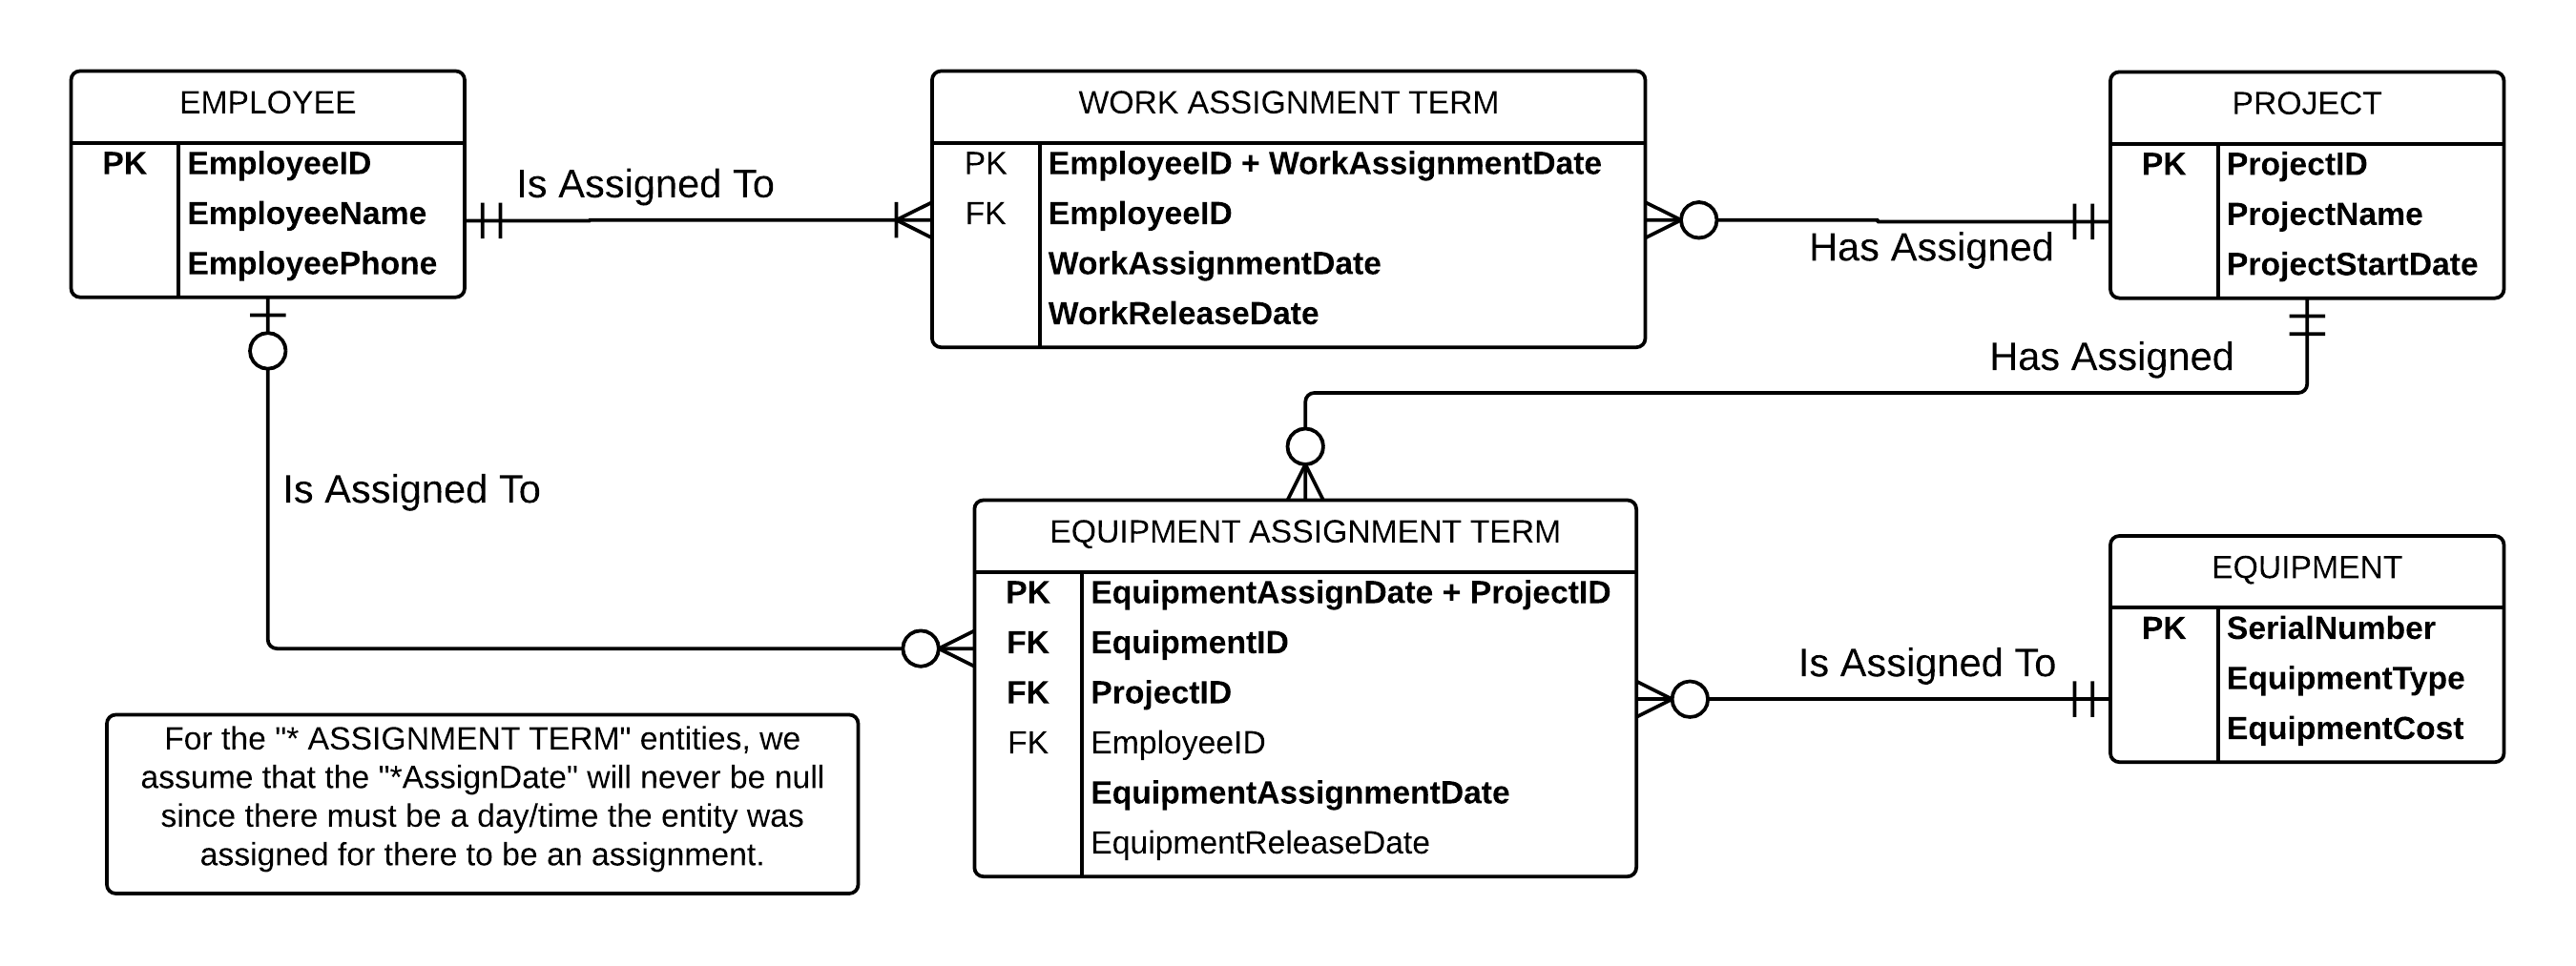
\includegraphics[width=.9\linewidth]{HW02_01-ERD}
    \caption{The solution ERD for Chemical Engineering Company's database.}
    \label{fig:chemeng}
  \end{figure}

\newpage
\section{ShapeShifters Fitness Center}

Design a database for ShapeShifters Fitness Center, a company that provides personal training. ShapeShifters plans to use this database to keep track of: customers and potential customers, membership type, trainers, training events (scheduled and completed), and notes and price related to a specific training event. Sample data for ShapeShifters is provided in the Excel workbook called “ShapeShiftersData” available as a link in the same cell where you found this assignment. Each row in the worksheet represents one personal training event conducted, or scheduled to be conducted, by a trainer at ShapeShifters. Here is some additional information about the sample data:
\begin{itemize}
  \item A customer has only one name and phone number.
  \item A customer who is a member has a membership typeID. It is possible for a customer to get training from ShapeShifters, but not be a member of the fitness center. If a customer is not a member (like Jim Beaker in the sample data) then the membership typeID is null for that customer.
  \item A membership type and membership monthly fee is related to a membership type.
  \item A trainer has a name.
  \item The hourly rate paid to a trainer is related to a trainer. A trainer only has one hourly rate.
  \item The training hourly price is related to a specific training event. The price may change for each event.
\end{itemize}

  \begin{figure}[h]
    \centering
    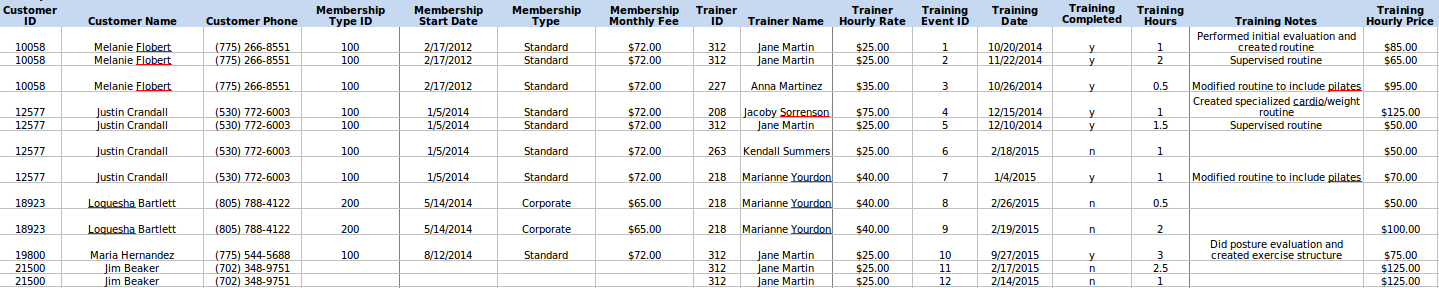
\includegraphics[width=.9\linewidth]{shapeshifter_data}
    \caption{The sample data for ShapeShifters Fitness Center.}
    \label{fig:chemeng}
  \end{figure}

\textit{Solution}:

  \begin{figure}[h]
    \centering
    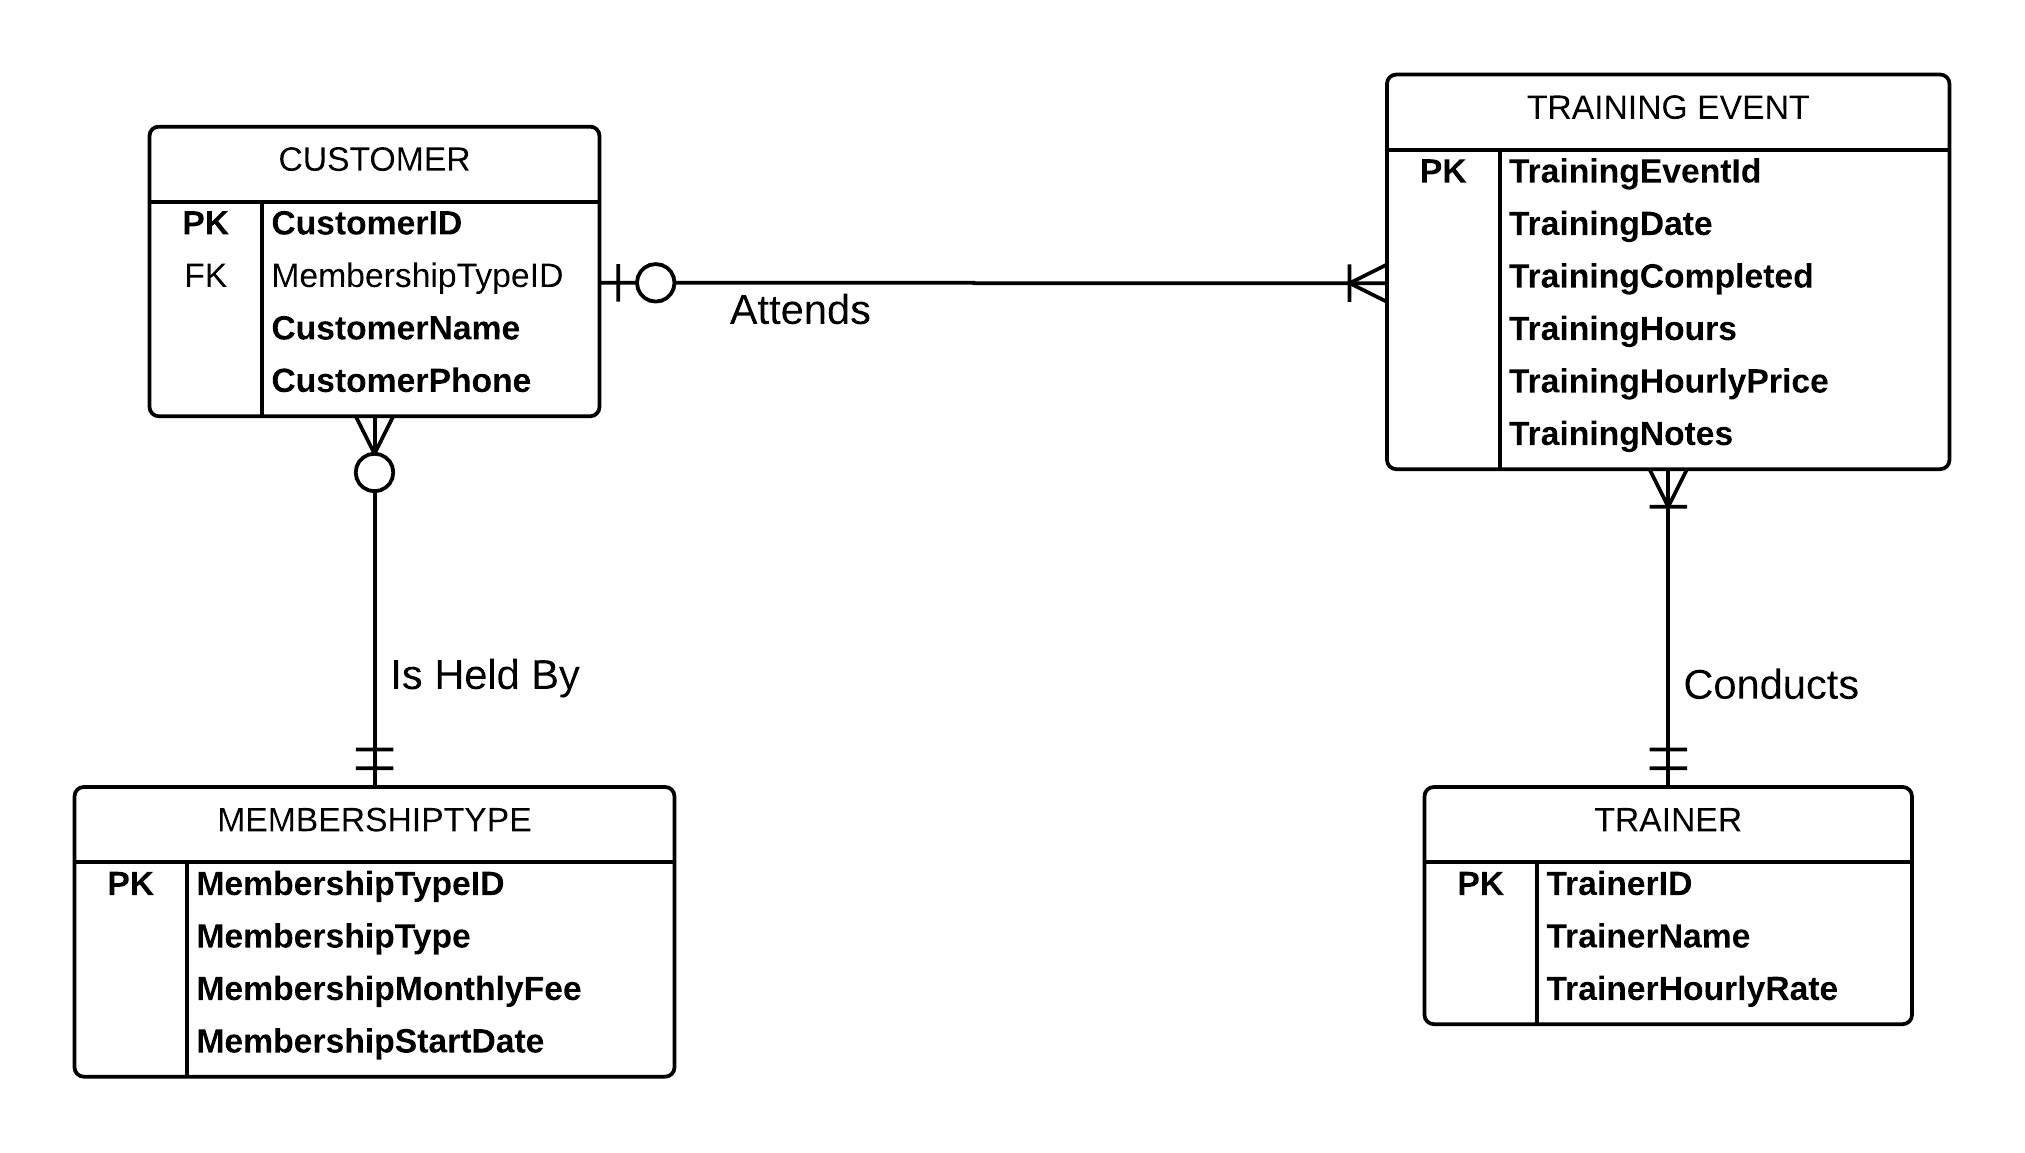
\includegraphics[width=.7\linewidth]{HW02_02-ERD}
    \caption{The solution ERD for ShapShifter's database.}
    \label{fig:shapeshifter}
  \end{figure}

\newpage
\section{The Hospital}

You have been asked to design a database for a single hospital (there is only one hospital – it is not part of a group of hospitals). The hospital wants to keep track of data about patients. The hospital wants to keep track of patient admittance, as well as patient treatment by health care professionals. Patients are admitted to the hospital by physicians, but physicians are only one kind of health care professional (HCPROF) at the hospital. Assume that the hospital has a large number of HCPROF’s, but they don’t need to differentiate between physicians and other types of HCPROF’s. Attributes of HCPROF include HCPROFID (identifier), type, and specialty. The hospital wants to keep track of the date a patient was admitted and also the admitting HCPROF. It is possible that a patient may be admitted to the hospital more than once. This is an example of “time stamping” data so that the data can be maintained over time. The hospital wants to keep the patients on file with the assumption that the patient may be admitted more than once and the hospital needs to know each different date that a patient was admitted. Attributes of PATIENT include patient\_id (identifier) and patient\_name. Any individual patient who is admitted must have exactly one admitting HCPROF, but an HCPROF may admit no patients or many patients. Once admitted, a given patient may be treated by no HCPROF’s, but could be treated by multiple HCPROFs. The particular HCPROF who admits a given patient may or may not treat that same patient. A particular HCPROF may treat any number of patients, or may not treat any patients. Whenever a patient is treated, the hospital records the details of the treatment (TREATMENTDETAIL). Attributes of TREATMENTDETAIL include date, time, and outcome. It is possible that more than one HCPROF participates in the same TREATMENTDETAIL for a patient. The hospital wants to keep track of all HCPROF’s who participate in a treatment. For each HCPROF who participates in a TREATMENTDETAIL, the hospital wants to record the notes from the HCPROF and the amount of time that the HCPROF spent on the treatment. For example, if three HCPROF’s participate in a single TREATMENTDETAIL for a single patient, the hospital wants to keep track of the notes and time spent for each of the three HCPROF’s.\\

\textit{Solution}:

  \begin{figure}[h]
    \centering
    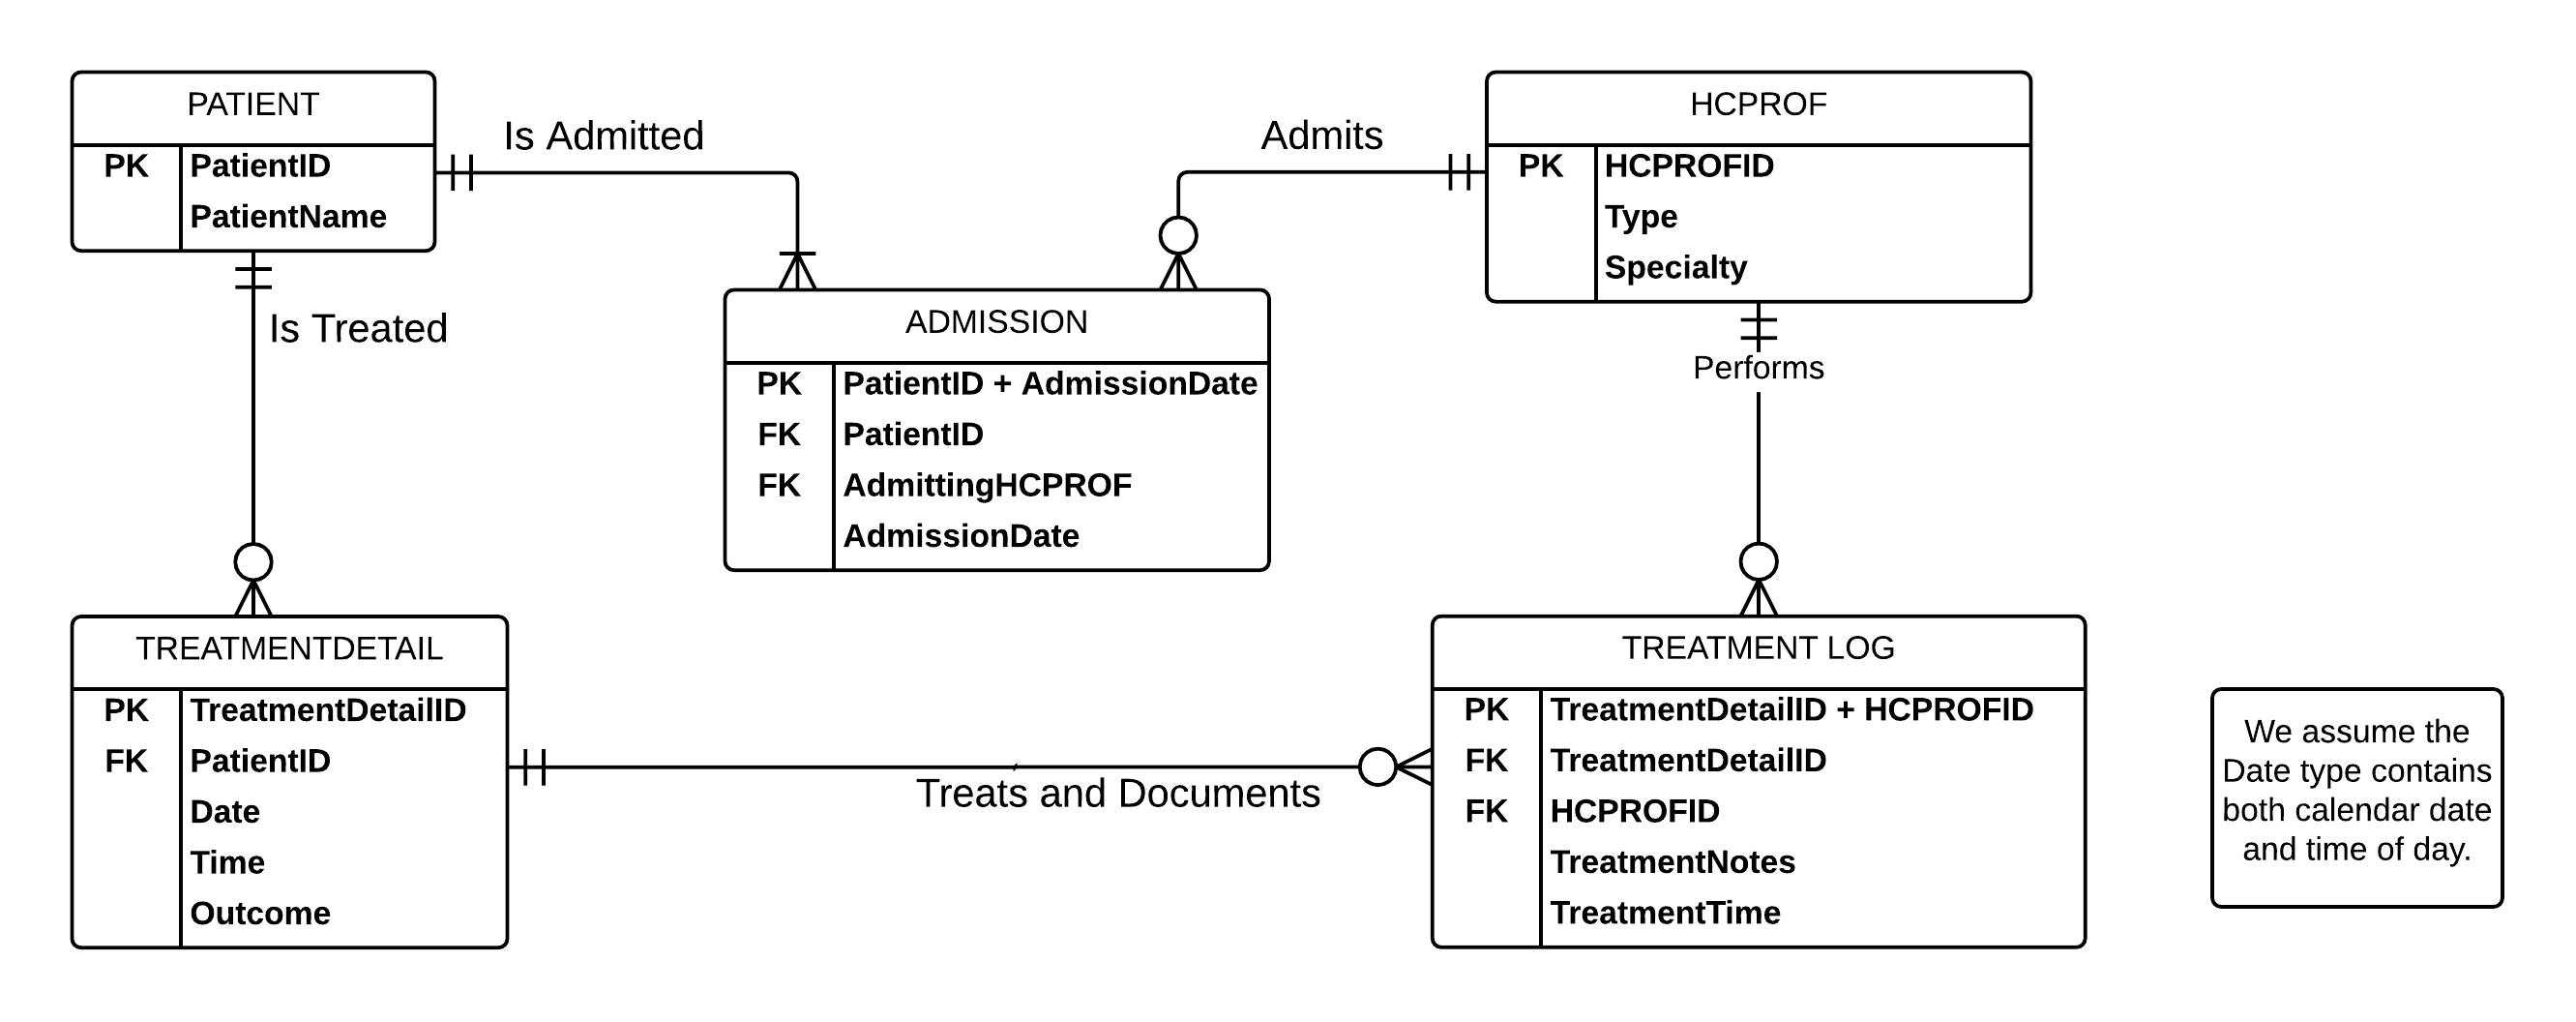
\includegraphics[width=.9\linewidth]{HW02_03-ERD}
    \caption{The solution ERD for the Hospital's database.}
    \label{fig:hospital}
  \end{figure}
  
\end{document}
